%=============================================================================
% SCRAPPED
%=============================================================================
% BACKGROUND
% This \LaTeX template is based on the ACM \texttt{sig-alternate} class. The layout is two-column text. Generally figures and tables only extend to one column width, e.g.\ Table \ref{tab-eg}, but it is possible to make them stretch over both columns using the \texttt{figure*} and \texttt{table*} environments. For an example, see Figure \ref{fig-eg}.

% \begin{table}
% \begin{tabular}{l||c||p{2cm}}
% \emph{Operating System} & \emph{Version} & \emph{Verdict} \\ \hline \hline
% Ubuntu & 12.04 & Everyone's favourite Linux, unless you grew up with RedHat \\ \hline
% Slackware & xxx & Pseudo-hacker's Linux, how often do you recompile your kernel? \\ \hline
% Mac OS & 10.7 & For people with more money than sense \\ \hline
% \end{tabular}
% \caption{\label{tab-eg}Single column table of figures}
% \end{table}

% \begin{figure*}
% \begin{center}
% \includegraphics[scale=0.3]{images/alice.pdf}
% \end{center}
% \caption{\label{fig-eg}An example figure stretching over two columns}
% \end{figure*}

\documentclass[../mpaper.tex]{subfiles}
\begin{document}

To understand Developer Experience, we first describe the importance of User Experience; it involves all aspects of the interaction between \textbf{the end-user} \& the product (usually an interface) \cite{experienceDefinitionUserExperience} representing the \textit{holistic} perspective of how a person feels about using a system. For this, interaction design becomes an essential part of any system involving studies of psychology, information architecture, user research and most importantly, Human-Computer Interaction (HCI). From the Machine Age, the end-users \& market have been important for the product to sell and succeed, so development of products tends to be user-driven/user-centered where a (fictional) persona's usability goals, characteristics, rationale \& motivations are determined. There have been recognised heuristics outlined for interface design \cite{experience10UsabilityHeurisitics} along with published articles in the International Organization for Standardization (ISO). ISO 9241\noteurl{https://www.iso.org/standard/52075.html} describes human-centered design as an approach to design systems that improve quality (of life) for users by 1) being comprehensive \& reducing training, 2) reducing discomfort and stress, 3) contributing towards sustainable objects without threatening life, and most importantly 4) \textbf{increasing the productivity and enhancing effectiveness \& efficiency of users and organisations} providing a competitive advantage. With this, User Experience (UX) design has become a large field with research and practitioners separate from User Interface (UI) design (like in UI/UX).

\subsubsection*{Developer Experience}

Developer Experience (DX) is user experience from a developer's point-of-view, i.e. the user is a person involved in the process of software development, so the persona can be known to have relatively higher technical knowledge and the products they use are involved in the development process. For example, text/source-code editors such as Vim\noteurl{https://www.vim.org/}, Emacs\noteurl{https://www.gnu.org/s/emacs/} and Sublime Text\noteurl{https://www.sublimetext.com/} are used by developers to view, edit and/or write code as a lower-level interaction with the computer in order to create relatively higher-level interfaces for end-users; enabling developers to easily use their software \& the editor would increase productivity and popularity in the market (we commonly see comparative discussions between Vim and Emacs and how keybindings are important), so Integrated Development Environments (IDE) aim to provide the essential facilities (such as source-code editor, build tools and debugger) in one program to maximize productivity and minimize friction.

% Why is Linux so popular with developers? Customisation and control.
Since the market is important for any product and its organisation, Developer Experience is a part of a wider field called Developer Relations (DevRel) \cite{bookFrameworkDeveloperRelations2021}, which also involves Developer Marketing \& Education, focusing on building and nurturing relationships between organisations and developers in terms of using a product so that both - the organisation and the developers - can benefit from each other; this can be seen similar to the field of Public Relations (PR) where the public is the developer, and so DevRel can also be seen as an area of marketing \& sales more than engineering \cite{communications8thDevRelSurvey2021}. The earliest DevRel program is known to be in the 1980s from Apple to influence developers to build applications for the Macintosh platform \cite{WhatDeveloperRelations2019}. Since then, large\footnote{Marketing \& DevRel requires funding so smaller organisations are not able to invest greatly} corporations such as \href{https://www.youtube.com/watch?v=Vhh_GeBPOhs}{Microsoft} \& Google have routinely organised programs and conferences for developers while DevRel only started to become mainstream over the last decade as more SaaS startups (like Twilio, Zendesk, and Intuit) started getting popular.

\subsubsection*{Rise of the Internet \& Open-Source}\label{sec:Background}%\label{subsubsec:the_internet}

Advancement in technology, especially over the last decade with the popularity of performant mobile devices with easily available fast internet, web development have a very high demand. Browsers (clients) only display HTML pages with CSS styling and JavaScript for interaction manipulation - their usage has increased and become essential. Large, complex websites with a lot of data (such as MySpace, Yahoo, Facebook) would use PHP hosted on expensive servers to render a client-compatible page, but that is now on a decline with the ability to run JavaScript outside the browser (and as a server or even serverless lambda function\noteurl{https://aws.amazon.com/lambda/}) with the introduction of (open-source) runtime engines (V8\noteurl{https://v8.dev/}) and environments (like Node.js\noteurl{https://nodejs.dev/} and Deno\noteurl{https://deno.land/}) over the decade; this allows developers to no longer learn PHP and develop web applications faster. Still, development would be further aided by frameworks that provided base implementation logic of a server, renderer, and/or webpages (like Express\noteurl{https://expressjs.com/}, Webpack\noteurl{https://webpack.js.org/} and Bootstrap\noteurl{https://getbootstrap.com/} respectively); so DevRel becomes essential for these technologies. While many tools embrace the open-source movement, it restricts them from stable, large funding that enables the (linear) marketing of their product; instead, they must rely on no-cost word-of-mouth referral systems (compounding growth) which can only be activated by good retention, so they focus on providing great developer experience and support/documentation.

While at the same time, tech giants like Facebook and Microsoft assign paid teams to create \& maintain their open-source solutions; this includes the revolutionary\noteurl{https://www.youtube.com/watch?v=8pDqJVdNa44} front-end JavaScript framework React(.js)\noteurl{https://react.dev/}, to help create complex pages easier and faster (also to move away from PHP), and back-end TypeScript\noteurl{https://typescriptlang.org/}, to eliminate human-errors \& frustrations in development with strict, extended code completion (like IntelliSense), and provide reliable production-ready applications despite non-compiled dynamic typing in JavaScript, respectively. Google has also led the development of the Angular\noteurl{https://angular.io/}(JS)\noteurl{https://angularjs.org/} framework, but its usage has been in great decline possibly due to bad DX with a closed ecosystem and strict code opinions.

Concurrently, indie developers that use the existing tools create new ones. Hick's law conveys that the time taken for a person to make a decision is directly proportional to the number of choices. React was also popularised for being unopinionated, but that gave developers too many options and styles to write code (such as class and functional components) so the codebase could become mixed and inconsistent. While Angular also had advantages, especially for enterprise applications, it was rather too opinionated and added constraints to developers' preferences. The third prominent JavaScript framework \textit{Vue}(.js)\noteurl{https://vuejs.org/} was created by an individual Evan You after using both frameworks to provide a middle-ground and also popularise the Single-File Component (SFC) architecture that was well-received by developers with easy DX; the same team from Vue developed Vite\noteurl{https://vitejs.dev/} as a faster, DX-focused alternative to Webpack for building (compiling) code for browsers as JavaScript also improved over-time with ESM\noteurl{https://developer.mozilla.org/en-US/docs/Web/JavaScript/Guide/Modules} (module) support; it made development better because of the fast \textit{Hot Module Replacement} (HMR) allowing changes to the code to be previewed (almost) instantly. These technologies, and their stories, show the difference between a poor developer environment (no IDE help, slow saves, manual refreshes, slow pipelines) and a great developer environment (fancy editor assistance, hot reloading, fast everything) proving that a good developer environment, good DX, makes the individual a better and more productive programmer \cite{WhatDeveloperExperience2020}.

Since 2016, the JavaScript community has had an annual developer survey\noteurl{https://survey.stackoverflow.co/2022/} that gathers developers' demographics, motivations and preferences. The graph in \autoref{fig:framework_retention} shows the developer relation for front-end frameworks showing Angular and React on the decline (along with Vue due to breaking changes in the framework), while Svelte, the new entry, made SFC more easy and performant. Along with that, Vite was the most adopted technology with the highest retention and interest in the two years of existence.

\begin{figure}[h]
    \centering
    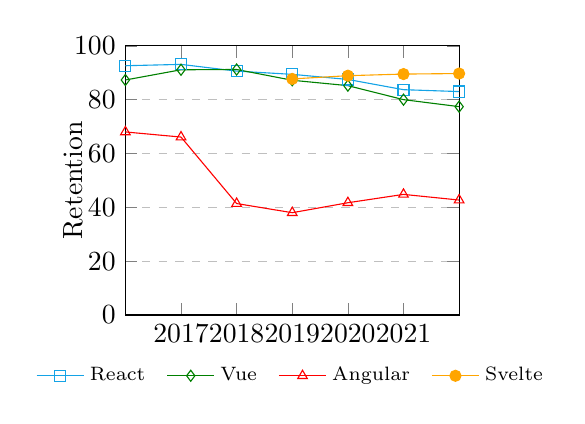
\begin{tikzpicture}
        \begin{axis}[width=0.48\textwidth, height=5cm, xlabel={Year}, ylabel={Retention}, y label style={at={(axis description cs:-0.1,.5)},anchor=south}, xmin=2016, xmax=2022, ymin=0, ymax=100, xtick={2017,2018,2019,2020,2021}, legend style={/tikz/every even column/.append style={column sep=0.2cm},at={(0.5,-0.15)},anchor=north,legend columns=-1,draw=none,font=\scriptsize}, ymajorgrids=true, grid style=dashed, xticklabel style={/pgf/number format/1000 sep=,}]
            \addplot[color=Cerulean, mark=square] coordinates {(2016,92.6)(2017,93.1)(2018,90.6)(2019,89.4)(2020,87.5)(2021,83.7)(2022,83)};
            \addplot[color=Green, mark=diamond] coordinates {(2016,87.3)(2017,91.1)(2018,91.2)(2019,87.2)(2020,85.2)(2021,80)(2022,77.4)};
            \addplot[color=Red, mark=triangle] coordinates {(2016,68)(2017,66.1)(2018,41.4)(2019,38)(2020,41.7)(2021,44.8)(2022,42.7)};
            \addplot[color=Orange, mark=*] coordinates {(2019,87.7)(2020,88.9)(2021,89.5)(2022,89.7)};
            % \addplot[color=CadetBlue,mark=*]coordinates {(2021,89.5)(2022,90.0)};

            \legend{React,Vue,Angular,Svelte}%,Solid}
        \end{axis}
    \end{tikzpicture}
    \caption{Retention over time for front-end frameworks}
    \label{fig:framework_retention}
\end{figure}

The main motivation for providing good DX is to activate the developer (the user) with the least friction so that they can get going with using the product without frustrations and are motivated to continue progressing with productivity. This includes developer portal, documentation, tools and utilities. For example, an API may automatically generate and safely store the authentication token by the logged-in session in the machine's browser and also provide live-demo documentation using the developer's token to different endpoints.

% \begin{figure}[h]
%     \centering
%     \begin{subfigure}{0.42\textwidth}
%         \frame{\includegraphics[width=\textwidth]{rapid-api-playground.png}}
%         \caption{RapidAPI}
%     \end{subfigure}
%     \vskip\baselineskip
%     \begin{subfigure}{0.18\textwidth}
%         \frame{\includegraphics[width=\textwidth]{webiny-api-playground.png}}
%         \caption{Webiny}
%     \end{subfigure}
%     \hfill
%     \begin{subfigure}{0.24\textwidth}
%         \frame{\includegraphics[width=\textwidth]{hygraph-api-playground.png}}
%         \caption{Hygraph}
%     \end{subfigure}
%     \caption{Example of Documentation API Playgrounds}
%     \label{fig:api_playground}
% \end{figure}

Stack Overflow is an established website in the computing science community \& industry, also created in the web-technology boom over the decade (and a billion-dollar company Stack Exchange), with over 20 million registered users posting 24 million questions with 35 million answers; referring to the site is a natural step in software engineering now with the usage of search engines like Google and SO showing as top-results. It has helped provide support and communities for technologies and frameworks. JavaScript is the most discussed topic on the site. They conduct an annual developer survey asking questions to understand the community. It reveals the most loved and most dreaded programming languages (see \autoref{fig:so_survey}) and a section on Developer Experience sharing the tools available within an organisation to aid developers; while more than 50\% had CI/CD and DevOps functions, only 38\% had a developer portal (listing tools and services) for their organisation and only 16\% had Innersource initiatives.

\begin{figure}[h]
    \centering
    \resizebox{0.48\textwidth}{!}{%
        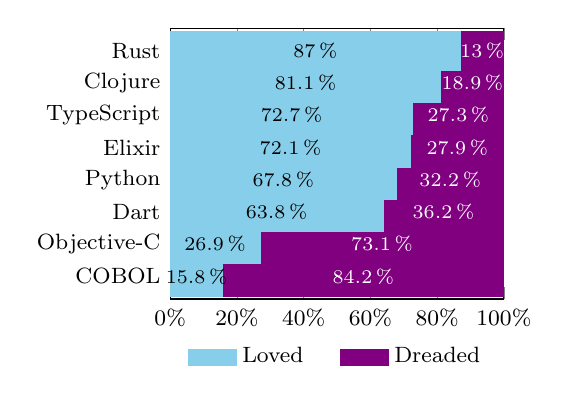
\begin{tikzpicture}
            \begin{axis}[
                    xbar stacked,
                    area legend,
                    legend style={/tikz/every even column/.append style={column sep=0.4cm},at={(xticklabel cs:0.5)},anchor=north,legend columns=5,draw=none,font=\footnotesize},
                    ytick=data,
                    tick label style={font=\footnotesize},
                    width=0.48\textwidth,
                    xticklabel={\pgfmathparse{\tick}\pgfmathprintnumber{\pgfmathresult}\%},
                    bar width=5mm,
                    y dir=reverse,
                    yticklabels={Rust,Clojure,TypeScript,Elixir,Python,Dart,Objective-C,COBOL},
                    xmin=0,
                    xmax=100,
                    nodes near coords={\pgfkeys{/pgf/fpu}\pgfmathparse{\pgfplotspointmeta}\pgfmathprintnumber{\pgfmathresult}\,\%},
                    nodes near coords style={font=\scriptsize, /pgf/number format/.cd,precision=1},
                    % grid style={line width=.01pt},
                ]
                % Loved
                \addplot[SkyBlue,fill=SkyBlue,text=black,
                    postaction={
                            % pattern=vertical lines
                        }] coordinates {(86.98, 0)(81.12, 1)(72.73, 2)(72.11, 3)(67.83, 4)(63.77, 5)(26.93, 6)(15.79, 7)};

                % Dreaded
                \addplot[Purple,fill=Purple,text=white,
                    postaction={
                            % pattern=horizontal lines
                        }] coordinates {(13.02, 0)(18.88, 1)(27.27, 2)(27.89, 3)(32.17, 4)(36.23, 5)(73.07, 6)(84.21, 7)};

                \legend{Loved,Dreaded}
            \end{axis}
        \end{tikzpicture}
    }
    \caption{Responses for programming languages}
    \label{fig:so_survey}
\end{figure}

\subsubsection*{Productivity}

The COVID-19 pandemic, aside from having vaccines being delivered in record time, saw software being released and updated in faster sprints; for example, video conferencing was necessary over lockdown, and Zoom\noteurl{https://zoom.us/} \& Microsoft Teams\noteurl{https://teams.com/} shipped with lots of bugs and minimum features that were fixed overtime with multiple releases. In such circumstances, companies aim to improve their resource allocation, process efficiency, and cost reduction, so they desire to employ developers with high productivity. Organisations tend to measure software productivity \cite{devanbuAnalyticalEmpiricalEvaluation1996} using automated metrics like source lines of code (SLOC) written \cite{barry1981software,conteSoftwareEngineeringMetrics1986,jonesProgrammingProductivity1985,walstonMethodProgrammingMeasurement1977,devanbuAnalyticalEmpiricalEvaluation1996}, function points \cite{albrecht1979measuring,computerstaffSoftwareMetricsGood1994}, changes request fulfilled \cite{cataldoSociotechnicalCongruenceFramework2008,millerHowWasYour2021}, and \textit{optionally filling timesheets manually which can be very vague}. These are highly objective (inaccurately) capturing a small part of a developer's work. The traditional definition of productivity (ratio between outputs over inputs \cite{morisioFrameworkBasedSoftware1999,pritchard1995productivity}) cannot be contrasted to software development as it typically involves creating new solutions \cite{trendowiczChapterFactorsInfluencing2009} for which developers may need to conduct tasks outside writing code; this includes being in meetings, researching technologies, reading documentation, and learning tools.

There could be a lot of effort put to make a commit of 3 additions and 2 deletions, and development should be aware of all human efforts so that it is acknowledged and future resources aren't wasted. Ensuring good productivity in a process ensures good development experience \cite{amabileProgressPrincipleUsing2011,graziotinFeelingsMatterCorrelation2015,meyerSoftwareDevelopersPerceptions2014,mullerStuckFrustratedFlow2015}. It is essential to recognise that developers are humans\noteurl{https://twitter.com/mahemoff/status/1947230411948032} and to include the hidden fourth-corner of The Project Management Triangle (by Barners in 1980) which is "\textit{Emotional Cost}".

\begin{figure}[h]
    \centering
    \begin{subfigure}{0.22\textwidth}
        \resizebox{\textwidth}{!}{%
            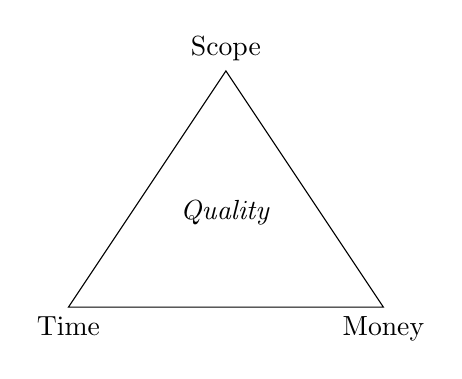
\begin{tikzpicture}
                \draw (0,0) node[anchor=north]{Time}
                -- (4,0) node[anchor=north]{Money}
                -- (2,3) node[anchor=south]{Scope}
                -- cycle;

                \draw (2,1.2) node{\textit{Quality}};
            \end{tikzpicture}
        }
    \end{subfigure}
    \hfill
    \begin{subfigure}{0.23\textwidth}
        \resizebox{\textwidth}{!}{%
            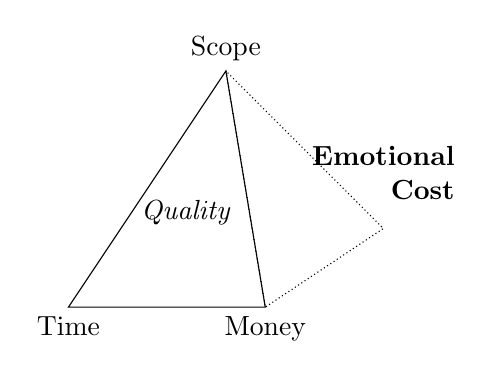
\begin{tikzpicture}
                \draw (0,0) node[anchor=north]{Time}
                -- (2.5,0) node[anchor=north]{Money}
                -- (2,3) node[anchor=south]{Scope}
                -- cycle;
                \draw (1.5,1.2) node{\textit{Quality}};
                \draw[densely dotted] (2,3) node[anchor=south]{}
                -- (2.5,0) node[anchor=north]{}
                -- (4,1) node[
                        anchor=south,
                        % text width=2cm,
                        label={[align=right, font=\bfseries]{Emotional\\Cost}}
                    ]{}
                % ]{\textbf{Emotional\\Cost}}
                -- cycle;
            \end{tikzpicture}
        }
    \end{subfigure}
    \caption{Project Management Triangle}
\end{figure}

\end{document}
